\documentclass[a4paper,twocolumn,11pt]{quantumarticle}
\pdfoutput=1
\usepackage[utf8]{inputenc}
\usepackage[english]{babel}
\usepackage[T1]{fontenc}
\usepackage{amsmath}
\usepackage{adjustbox}
\usepackage{hyperref}
\usepackage{pgfplots}
\usepackage{tikz}
\usetikzlibrary{shapes.geometric, positioning}
\usetikzlibrary{arrows.meta, decorations.pathmorphing}
\usepackage{lipsum}
\usepackage{caption}
\captionsetup{width=0.8\textwidth}
\usepackage{braket}
\usepackage{multirow}
\usepackage[utf8]{inputenc}
\usepackage[english]{babel}
\usepackage[T1]{fontenc}
\usepackage{amsmath}
\usepackage[numbers,sort&compress]{natbib}
\usepackage{hyperref}
\usepackage{amsfonts} 
\usepackage[numbers]{natbib}
%\usepackage[backend=bibtex]{biblatex}
%\addbibresource{bibliography.bib}
\newtheorem{theorem}{Theorem}
\pgfplotsset{compat=1.18}

\begin{document}

\title{Qubit-Based Framework for Quantum Machine Learning: Bridging Classical Data and Quantum Algorithms}

\author{Bhavna Bose}
\affiliation{Mukesh Patel School of Technology Management and Engineering, SVKM's NMIMS}
\email{bhavna.bose@nmims.edu}
\orcid{0009-0009-8260-7853}
\author{Saurav Verma}
\affiliation{Mukesh Patel School of Technology Management and Engineering, SVKM's NMIMS}
\email{saurav.verma@nmims.edu}
\orcid{0000-0001-5343-6826}

\maketitle

\begin{abstract}
  This paper dives into the exciting and rapidly growing field of quantum computing, explaining its core ideas, current progress, and how it could revolutionize the way we solve complex problems. It starts by breaking down the basics, like qubits, quantum circuits, and how principles like superposition and entanglement make quantum computers fundamentally different—and far more powerful for certain tasks—than the classical computers we use today. We also explore how quantum computing deals with complex problems and why it’s uniquely suited for challenges classical systems struggle to handle.  
A big part of this paper focuses on Quantum Machine Learning (QML), where the strengths of quantum computing meet the world of artificial intelligence. By processing massive datasets and optimizing intricate algorithms, quantum systems offer new possibilities for machine learning. We highlight different approaches to combining quantum and classical computing, showing how they can work together to produce faster and more accurate results. Additionally, we explore the tools and platforms available—like TensorFlow Quantum, Qiskit, and PennyLane—that are helping researchers and developers bring these theories to life.  
Of course, quantum computing isn’t without its hurdles. Challenges like scaling up hardware, correcting errors, and keeping qubits stable are significant roadblocks. Yet, with rapid advancements in cloud-based platforms and innovative technologies, the potential of quantum computing feels closer than ever. This paper aims to offer readers a clear and comprehensive introduction to quantum computing, its role in machine learning, and the immense possibilities it holds for the future of technology.
\end{abstract}

\section{Introduction}\label{sec1}
Machine learning has transformed the data analytics industry like never before. With availability of a variety of data in large volumes at high velocity, i.e., 'Big Data', significant insights can be drawn. As the volume of data increases, so does the difficulty in processing it. There is a need for systems that can efficiently process large data sets, using complex algorithms, in real time and with high accuracy. In our fast-paced world, the industry is driven by the urge to speed up processed and make them more efficient and safe. 
Quantum computing provides a platform to achieve this, with a few caveats! Quantum physics has been around for quite some time. However, Shor's algorithm \cite{shor1994algorithms} catapulted the interest in Quantum Computing. Fig. \ref{fig:QuantumComputingTimeline} shows the progress of Quantum research from 1982 to 2024. 

Quantum computing research has grown in leaps and bounds.Google and IBM are the two front runners in this Quantum race. In just a couple of years IBM has successfully developed a quantum computer capable of running up to 5000 two qubit gate operations. \cite{ibmQuantumDelivers} . In December 2024, Google launched their breakthrough 105 Qubit Quantum chip called Willow.\cite{acharya-2024}. This latest development has tackled a very important challenge in Quantum computing of error reduction and decoherence as we increase the number of Qubits. These advancements have accelerated the growth in Quantum research and development.

\begin{figure*}[t]
\centering
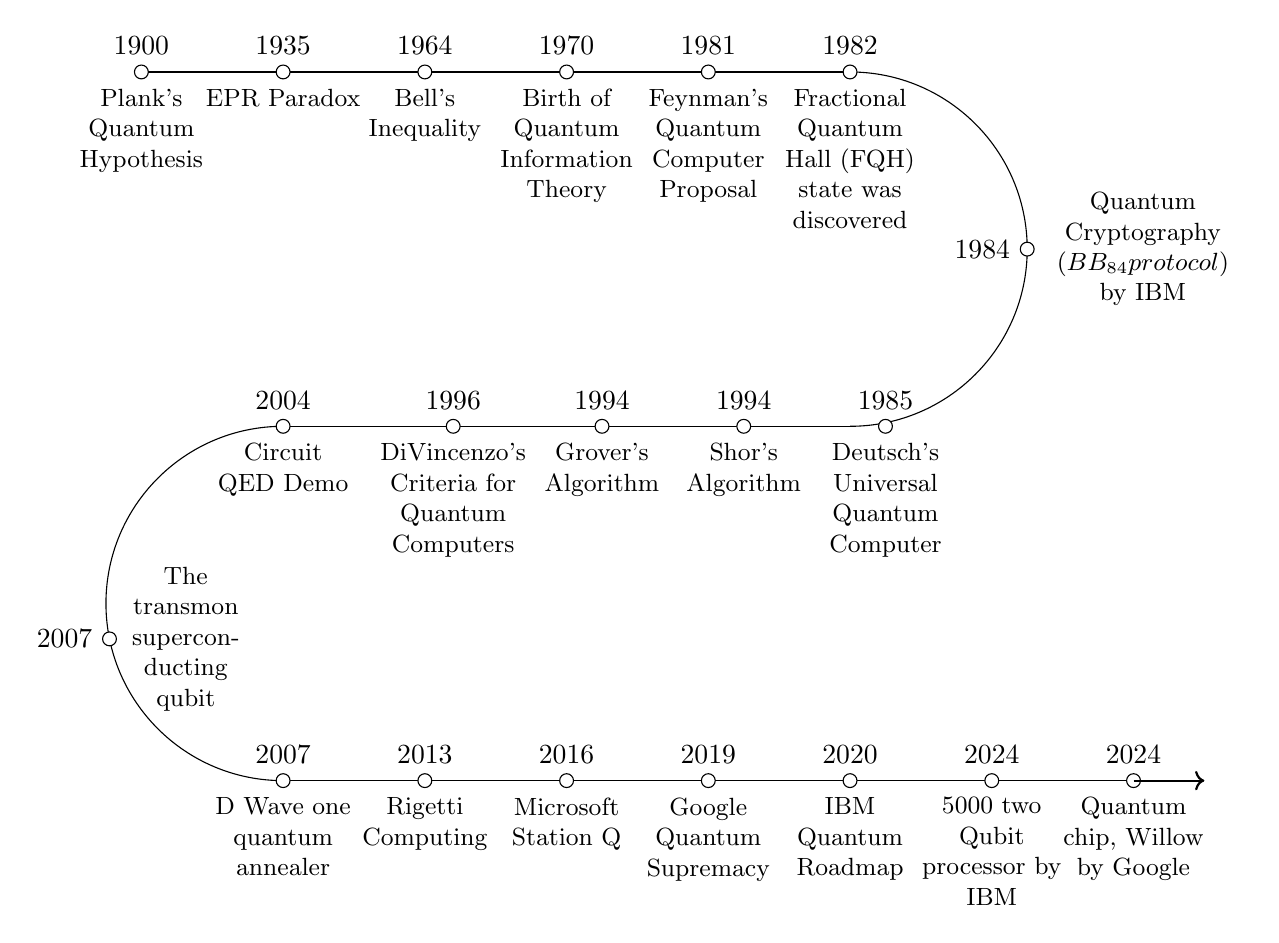
\begin{tikzpicture}[scale=0.9]
% Define a reusable small circle node style
    \tikzstyle{smallcircle} = [circle, draw, fill=white, minimum size=5pt, inner sep=0pt]
    
    \draw (0,10)  - - (10,10); %top line
    \draw (2.0,5)  - - (10,5);   %middle line  
    \draw (2,0)  - - (15,0);  % bottom line 
    \draw (10,10) arc [start angle=90, end angle=0, radius=2.5cm];  
    \draw (12.5,7.5) arc [start angle=360, end angle=270, radius=2.5cm]; 
   \draw (2,5) arc [start angle=90, end angle=270, radius=2.5cm]; 
    
    % Place a small circle node
   \node[smallcircle , 
    label=below:{\parbox{2cm}{\centering \small Plank's Quantum Hypothesis}}, 
    label=above:{1900}] at (0,10) {};
    
    \node[smallcircle, 
    label=below:{\parbox{2cm}{\centering \small EPR Paradox}}, 
    label=above:{1935}] at (2,10) {};
    
    \node[smallcircle , 
    label=below:{\parbox{2cm}{\centering \small Bell's Inequality}}, 
    label=above:{1964}] at (4,10) {};

    \node[smallcircle , 
    label=below:{\parbox{2cm}{\centering \small Birth of Quantum Information Theory}}, 
    label=above:{1970}] at (6,10) {};

    \node[smallcircle , 
    label=below:{\parbox{2cm}{\centering \small Feynman's Quantum Computer Proposal}}, 
    label=above:{1981}] at (8,10) {};

    \node[smallcircle , 
    label=below:{\parbox{2cm}{\centering \small  Fractional Quantum Hall (FQH) state was discovered }}, 
    label=above:{1982}] at (10,10) {};

    \node[smallcircle , 
    label=left:{1984},
    label=right :{\parbox{2.5cm}{\centering \small Quantum Cryptography $(BB_{84} protocol)$ by IBM}} ] at (12.5,7.5) {};
    
    \node[smallcircle , 
    label=below:{\parbox{2cm}{\centering \small Deutsch's Universal Quantum Computer}}, 
    label=above:{1985}] at (10.5,5) {};
    
    \node[smallcircle, 
    label=below:{\parbox{2cm}{\centering \small Shor's Algorithm}}, 
    label=above:{1994}] at (8.5,5) {};
    
    \node[smallcircle , 
    label=below:{\parbox{2cm}{\centering \small  Grover's Algorithm}}, 
    label=above:{1994}] at (6.5,5) {};

    \node[smallcircle , 
    label=below:{\parbox{2cm}{\centering \small DiVincenzo's Criteria for Quantum Computers}}, 
    label=above:{1996}] at (4.4,5) {};

    \node[smallcircle , 
    label=below:{\parbox{2cm}{\centering \small Circuit \\QED Demo}}, 
    label=above:{2004}] at (2,5) {};
        
    \node[smallcircle , 
    label=left:{2007},
    label=right :{\parbox{1.5 cm}{\centering \small The transmon superconducting qubit}} ] 
    at (-0.45,2) {};
    
    \node[smallcircle, 
    label=below:{\parbox{2cm}{\centering \small D Wave one quantum annealer}}, 
    label=above:{2007}] at (2,0) {};
    
    \node[smallcircle , 
    label=below:{\parbox{2cm}{\centering \small Rigetti Computing}}, 
    label=above:{2013}] at (4,0) {};

    \node[smallcircle , 
    label=below:{\parbox{2cm}{\centering \small Microsoft Station Q}}, 
    label=above:{2016}] at (6,0) {};

    \node[smallcircle , 
    label=below:{\parbox{2cm}{\centering \small Google Quantum Supremacy}}, 
    label=above:{2019}] at (8,0) {};

    \node[smallcircle , 
    label=below:{\parbox{2cm}{\centering \small IBM Quantum Roadmap}}, 
    label=above:{2020}] at (10,0) {};
    \node[smallcircle , 
    label=below:{\parbox{2cm}{\centering \small 5000 two Qubit processor by IBM}}, 
    label=above:{2024}] at (12,0) {};

    \node[smallcircle , 
    label=below:{\parbox{2cm}{\centering \small Quantum chip, Willow by Google   }}, 
    label=above:{2024}] at (14,0) {};
    \draw[->, thick] (14,0) -- (15,0); % Arrow from (0,0) to (1,0)
     
\end{tikzpicture}
\centering
\caption{Quantum computing timeline}  
\label{fig:QuantumComputingTimeline}
\end{figure*}

Consider the performance of an algorithm as a function of the amount of time spent in solving the problem. As size of the input increases, high degree polynomial functions grow much slower than quadratic functions as shown in Fig \ref{fig:ComplexityComparisio}. Quantum systems provide speedups in this area.

\begin{figure}[h!]
\centering
    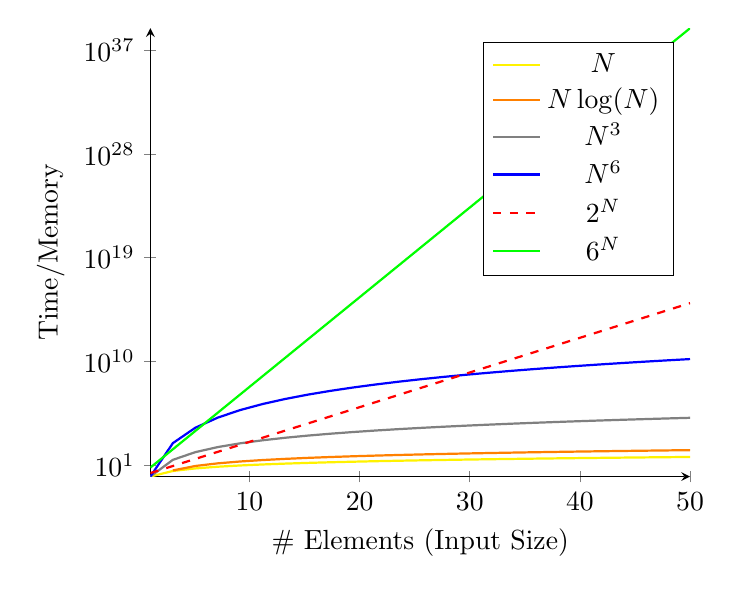
\begin{tikzpicture}
    \begin{axis}[
        axis lines = left,
        xlabel={\# Elements (Input Size)},
        ylabel={Time/Memory},
        ymode=log,
        legend pos=north east,    
        ]
    % Plot for N
    \addplot[yellow, thick, domain=1:50] {x};
    \addlegendentry{$N$}

    % Plot for N log(N)
    \addplot[orange, thick, domain=1:50] {x * ln(x)};
    \addlegendentry{$N \log(N)$}

    % Plot for N^2
    \addplot[gray, thick, domain=1:50] {x^3};
    \addlegendentry{$N^3$}

    % Plot for N^5
    \addplot[blue, thick, domain=1:50] {x^6};
    \addlegendentry{$N^6$}

    % Plot for 2^N
    \addplot[red, dashed, thick, domain=1:50] {2^x};
    \addlegendentry{$2^N$}

    % Plot for 5^N
    \addplot[green, thick, domain=1:50] {6^x};
    \addlegendentry{$6^N$}

    \end{axis}
    \end{tikzpicture}
    \caption{\parbox{0.4\textwidth}{\centering Comparison of time complexities based on number of inputs}}

    \label{fig:ComplexityComparisio}
\end{figure}

Classical systems store single information in a single bit i.e. 0 or 1. In contrast, quantum computers store information in qubits shown using the Dirac notation $ ket\psi$ written as $\ket{\psi}$. Each single qubit stores information about two states 0 and 1. However, on measurement, the qubit collapses to a single state i.e. 0 or 1. This means that in the intermediate process fewer qubits (N) can be used to process more ($2^N$)data.  All this is possible due to the duality of a quantum particle. 

This does not mean that classical computers will become obsolete. It is quite the opposite! The current research (as we will see the next section) is working on a symbiotic interaction between Quantum computers and Classical computers. Also as seen from Fig. \ref{fig:ComplexityComparisio}, quantum computing offers speedups for a particular class of problems. Each processing paradigm has its strength and by harnessing the strength of both systems, solutions of traditionally unsolvable problem can be attempted.

Just as quantum computing offers unique solutions to many unsolvable problems, quantum computing faces its unique challenges. \cite{10167529}, discusses the many challenges faced in the development of quantum computing based systems. These include hardware scalability, decoherence, and limited gate operations to name a few. Even with the tremendous work done in the development of quantum hardware by industry giants like IBM and Google, we are at least half a decade away before practical quantum systems will be available. 

\subsection{Related Literature}\label{subsec2}

The work done in \cite{bib28,bib29,bib30} gives an idea about different applications of machine learning, quantum information processing and the overlap between these two fields. For those seeking an entry point into the topics of Quantum Machine Learning (QML), \cite{bib31} serves as a valuable resource, while \cite{bib32} emphasizes algorithmic complexity and theoretical foundations through illustrative examples of QML techniques.

Further exploration into Quantum Neural Networks (QNN) is provided by \cite{bib33} and \cite{bib34}, which compare key QNN architectures, summarize their characteristics, and offer broader context within this domain. Additionally, \cite{bib35} demonstrates examples of quantum enhancements to  Machine Learning and Artificial Intelligence. Among introductory texts, the monograph by \cite{bib36} stands out as the most comprehensive resource, presenting significant discoveries in Quantum Machine Learning alongside a thorough introduction to both classical machine learning and quantum computing. Similarly, \cite{bib37} delves into well-established techniques, offering a detailed overview of the field.

A unique perspective is provided by \cite{bib38}, which explores QML's applications in robotics while also addressing classical QML concepts. Recent works have begun to propose specific application scenarios for QML. For instance, \cite{bib39} discusses how novel QNN architectures could address numerical challenges in finance, while \cite{bib40} examines the potential of quantum neural networks to enhance medical image recognition. Physics remains the most prominent area for QML applications, with \cite{bib41} offering a comprehensive review. Conversely, other cross-disciplinary applications have seen less significant contributions from QML, as noted by \cite{bib42}.

This work aims to an introduction to Quantum Machine Learning (QML). It covers foundational concepts, classical Quantum approaches integrating the existing systems with Quantum mechanisms, a proposed framework for implementing QML and suggesting resources for further exploration. Rather than striving for exhaustive coverage, the goal is to equip readers with sufficient background and guidance for deeper study.

This paper is organized as follows:  Section 2 introduces the basic concepts of quantum computing starting from Qubits till problem complexity. Section 3 discusses quantum computation with an introduction to Quantum  Circuits and their modeling. Section 4 is briefly discusses the steps involved in machine leaning, while Section 5 dives into quantum machine learning discussing the phases/steps to collaboratively use classical and quantum techniques. Section 6 discusses an implementation framework for of Quantum machine learning algorithms. Section 7 gives an overview of some quantum computing platforms available currently. Finally, Section 8 concludes the paper.

\section{Introduction to Quantum Computing}\label{sec2}
 In this section we will discuss the building block of Quantum systems, Qubits and the problem types which can be solved using the Quantum approach.
 \subsection{Qubits }\label{subsec2.1}
Qubits, are the basic building block of a quantum computing system. Qubits in quantum computers are analogous to bits in classical systems. Qubits are quantum particles and can be implemented using many physical particles like superconducting qubits, trapped ion qubits, quantum dots, photons, neutral atoms to name a few.

The different types of qubits used in quantum computing today are listed below:
\begin{itemize}
    \item Superconducting qubits: Superconducting materials like aluminum, niobium and tantalum are used to make the qubits. As extremely low temperatures, they enable fast and fine tuned computations.
    \item Trapped ion qubits: Qubits implemented as trapped ion particles can stay for longer periods without being disrupted by environmental noise and less errors in measurements.
    \item Quantum dots: they are nanoscale semiconductor particles. The electron in a Quantum Dot and confined in a very small three dimensional space making their energy levels discrete and measurable. 
    \item Photons: Photons are light particles which exhibit the phenomena of entanglement and superposition. Also, due to their weak interactions with surrounding environments they more immune to noise.
    \item Neutral atoms: Neutral atoms are atoms with equal number of electrons and protons, making them stabe for quantum communications. Quantum information is encoded in the internal states of these atoms.
\end{itemize}

Table \ref{tab:Qubittechnology} gives a summary of the different types of qubits and the companies building Quantum Processing Units (QPUs) using that technology.
\begin{table*}[t]
    \centering
    \caption{Qubit technology and Companies working on building QPUs using that technology.}
    \begin{tabular}{|l|l|}
    \hline
        \multirow{4}*{Superconducting qubits}&	IBM built the Eagle quantum computer with 127 qubits. \cite{bib5} \\
        &Google's Sycamore \cite{bib6}\\
        &Rigetti's Aspen-M-2 \cite{bib7}\\
        &QuantWare's built Crescendo and Soprano \cite{bib8}\\
        \hline

        \multirow{4}*{Trapped ion qubits}&	Quantinuum \cite{bib9}  \\
        &IonQ \cite{bib10}\\
        &Alpine Quantum Technologies \cite{bib11} \\
        &Oxford Ionics \cite{bib12}\\
        \hline
        \multirow{3}*{Quantum dots}&	Diraq \cite{bib13}   \\
        &Quobly \cite{bib14} \\
        &Quantum Motion \cite{bib15} \\
        \hline
        
        \multirow{4}*{Photons}&	Xanadu \cite{bib16}  \\
        &ORCA Computing \cite{bib17} \\
        &QuantumComputing Inc \cite{bib18}  \\
        &PsiQuantum \cite{bib19} \\
        \hline

        \multirow{4}*{Neutral atoms}&	Pasqal \cite{bib20}    \\
        & Atom Computing \cite{bib21}  \\
        &QColdQuanta \cite{bib22}  \\
        &QuEra \cite{bib23}  \\
        \hline
    \end{tabular}
    
    \label{tab:Qubittechnology}
\end{table*}


The spin and amplitude of the qubits carry information. To achieve this, the qubits have to be kept at very low temperatures, just above absolute zero (-459 degrees Fahrenheit), to be able to control their behavior (i.e. spin and amplitude). The main challenge to quantum computing is the difficulty in  maintaining such low temperatures. Even with a slight increase in temperature, the quantum particle (qubit) with change its state i.e. loose its value also called decoherence.\cite{bib4} Classical bits do not loose their information i.e they maintain their state over time. However, qubits loose their state very quicky i.e. loose coherence in less that 300$\mu s$  !\cite{Bal2024-vb} The low coherence implies that all computations must be completed before the qubit becomes decoherent. Decoherence forces the developers to create circuits and algorithms which will come to the final result very fast and accurately which aligns to the need of the the consumers too. It is a win-win situation !

\subsection{Classical Vs Quantum Complexity}
As discussed in the previous section, problems which can be solved efficiently with the classical computers, do not require to migrate to the more computationally expensive quantum systems. Then the question arises , which kind of problems are apt for quantum computations ? 
To answer the question, computational complexity of the problems needs to be explored. This section will discuss the different computation complexity classes. Computational complexity refers to the time and space required to compute a problem which is normally a function of the number of inputs i.e. input size.
Fig. \ref{fig:complexity_classes} shows the set of decision problems that require a certain amount of time and space.
\begin{itemize}
    \item Exponential Space Problems (EXPSPACE) : The space required to solve problems in this class is an exponential fuction of the number of inputs.
    \item Exponential Time Problems (EXPTIME) : The time required to solve  problems in this class is an exponential fuction of the number of inputs.
    \item Polynomial Space Problems (PSPACE) : The space required to solve problems in this class is a polynomial function of the number of inputs.
    \item Polynomial time problems (P ): Problems in this class can be solved in polynomial time as the input size increases.
    \item Non deterministic Polynomial time Problems (NP): Problems in the category cannot be solved in polynomial time. However, a solution to these problems can be verified in polynomial time.
    \item NP-complete problems: Problems in this class are the most difficult problems in NP and have no known polynomial solution. This is where famous problems like the traveling salesman and the game Soduku live.
    \item Bounded-error Polynomial Problems (BPP):  which can be solved within some error threshold by a probabilistic classical computer in polynomial time.
    \item Bounded-error Quantum Polynomial Problems (BQP): This is the quantum equivalent of BPP. It is the class of decision problems solvable by a quantum computer in polynomial time with a small chance of error.
\end{itemize}

\begin{figure*}[t]
    \centering
    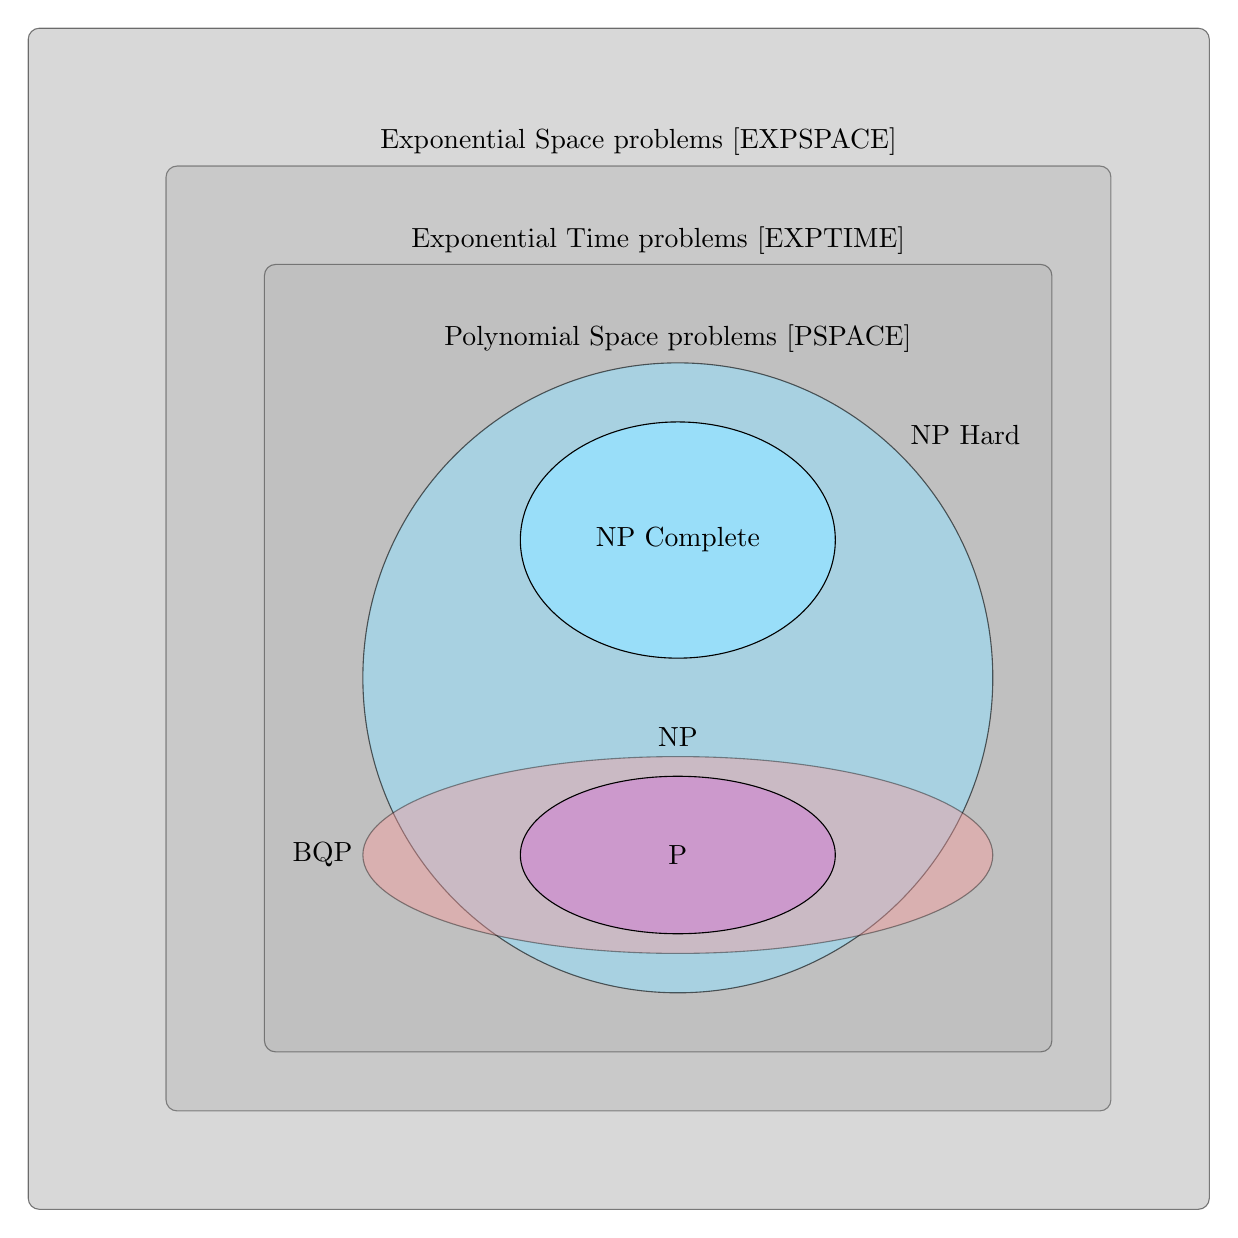
\begin{tikzpicture}[node distance=2cm]
    \tikzstyle{outerBBox} = [rectangle, rounded corners, minimum width=15cm, minimum height=15cm,text centered, draw=black, fill=black!30]
    \tikzstyle{outerBox} = [rectangle, rounded corners, minimum width=5cm, minimum height=7cm,text centered, draw=black, fill=red!30]
    \tikzstyle{innerBox} = [rectangle, rounded corners, minimum width=3cm, minimum height=1cm,text centered, draw=black, fill=blue!30]    
    \tikzstyle{Encircle} = [ellipse, minimum width=4cm, minimum height=2cm,text centered, draw=black, fill=cyan!40]
    \tikzstyle{arrow} = [thick,->,>=stealth]
    \node (ExpSpace) [outerBBox, opacity=0.5] at (0,0) {};
    \node (ExpTime) [outerBBox, label = above:{Exponential Space problems [EXPSPACE]}, opacity=0.4,minimum width=12cm, minimum height=12cm] at(0.25,-0.25) {};
    \node (PSpace) [outerBBox, label = above:{Exponential Time problems [EXPTIME]}, opacity=0.4,minimum width=10cm, minimum height=10cm] at(0.5,-0.5) {};
    \node (NPHard) [Encircle, 
                    label = above:{Polynomial Space problems [PSPACE]}, 
                    label=above right:{NP Hard},
                    opacity=0.6,minimum width=8cm, minimum height=8cm] at(0.75,-0.75) {};
    \node (NPComplete) [Encircle, 
                        opacity=1,
                        minimum width=4cm, 
                        minimum height=3cm,
                        ] at(0.75,1) {NP Complete};
    \node (BQP) [Encircle, opacity=0.4,minimum width=8cm, minimum height=2.5cm, fill=red!40, label=left:BQP,
    label=above:NP] at(0.75,-3) {};
    \node (PProblems) [Encircle, opacity=1,minimum width=4cm, minimum height=2cm, fill=violet!40] at(0.75,-3) {P};
    \end{tikzpicture} 
    
    \caption{Complexity Classes}\label{fig:complexity_classes}
\end{figure*}

\section{Quantum Logic}\label{sec3}
Quantum computing paradigm has certain core differences which makes it attractive. Due to the concepts of entanglement, superposition and superdense coding, quantum algorithms provide significant speedups to solve problems considered unsolvable earlier.
As opposed to bits, qubits can be evaluated to a 0 or a 1 based on the probability of geting the two values, i.e. a qubit is a linear function of 0 and 1 values. A qubit is represented by the equation Eq. \ref{eg:qubit}

\begin{equation}
    \ket{\psi} = \alpha \ket{0} + \beta\ket{1}
    \label{eg:qubit}
\end{equation}

where $\alpha, \beta \in \mathbb{C}$ are the popabilites of evaluating a qubit to 0 or 1 repectively. Thus $|\alpha|^2 + |\beta|^2 = 1$.  This means that during the intermediate computations, a qubit can be in a combination of $\ket{0}$ or $\ket{1}$ . Once measured, the Qubit will evaluate to either a 0 or 1 classical bit value. 

In an $n$-qubit system, there are $2^n$ probability amplitudes, which might suggest an enormous amount of information. The reality is that the measurements we can perform limit how much information we can actually extract. This idea is captured by Holevo's bound, which tells us that $n$ qubits can encode, at most, $n$ bits of information. \cite{bib25}.

\subsection{Quantum Circuits}\label{sec4}

Classical computations are performed by applying logic gates to the input bits. The logic gates transform the state of the bits based on certain rules. 

Analogously, gates are applied to qubits to perform certain computations and give results.

Much like classical logic gates, a quantum logic gate transforms, the input $A$ to $A'$ based on a transformation function applied to it through the logic gate. We usually denote a quantum state as $\ket{\psi} = \alpha \ket{0} + \beta\ket{1}$. When the quantum logic gate is applied to the quantum input state $\ket{\psi}$, it transforms to  $\ket{\psi'} = \alpha \ket{0'} + \beta\ket{1'}$ . As this is a valid quantum state, the condition $|\alpha'|^2 + |\beta'|^2 = 1$ is satisfied. \cite{bib36}. 

 Listed in Table. \ref{tab:quantum_gates}. are few quantum gates with their symbols and transformation matrices.

\begin{table*}[t]
    \centering
    \caption{Quantum Gates, Symbols, Matrices and Resultant Equation\\Input Qubit is $\ket{\psi}=\alpha\ket{0}+\beta\ket{1}$}
    \begin{tabular}{|c|c|c|c|}
        \hline
        \textbf{Gate Name} & \textbf{Symbol} & \textbf{Matrix Representation} &\textbf{Equation} \\ \hline
      
        Hadamard & 
        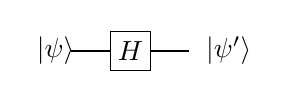
\begin{tikzpicture}
            \draw  (0,0) rectangle (0.5,0.5);
            \node at (0.25,0.25) {$H$};
            \draw[thick] (-0.5,0.25) -- (0,0.25);
            \draw[thick] (0.5,0.25) -- (1,0.25);
            \node at (-0.7,0.25) {$\ket{\psi}$};
            \node at (1.5,0.25) {$\ket{\psi'}$};
        \end{tikzpicture}
       
        & 
        $\frac{1}{\sqrt{2}} 
        \begin{bmatrix} 
        1 & 1 \\ 
        1 & -1 
        \end{bmatrix}$ 
        & 
        $\ket{\psi'} = 
        \frac{\alpha + \beta}{\sqrt{2}}\ket{0} + \frac{\alpha - \beta}{\sqrt{2}}\ket{1}$
        
        \\ \hline

        Pauli-X & 
        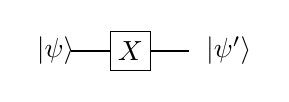
\begin{tikzpicture}
            \draw  (0,0) rectangle (0.5,0.5);
            \node at (0.25,0.25) {$X$};
            \draw[thick] (-0.5,0.25) -- (0,0.25);
            \draw[thick] (0.5,0.25) -- (1,0.25);
            \node at (-0.7,0.25) {$\ket{\psi}$};
            \node at (1.5,0.25) {$\ket{\psi'}$};
        \end{tikzpicture}
            
        
         & 
        $\begin{bmatrix} 
        0 & 1 \\ 
        1 & 0 
        \end{bmatrix}$ & 
         $\ket{\psi'} = \alpha\ket{1} + \beta\ket{0}$ 
         \\ \hline

        Pauli-Y & 
        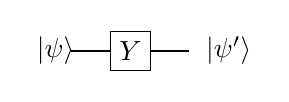
\begin{tikzpicture}
            \draw  (0,0) rectangle (0.5,0.5);
            \node at (0.25,0.25) {$Y$};
            \draw[thick] (-0.5,0.25) -- (0,0.25);
            \draw[thick] (0.5,0.25) -- (1,0.25);
            \node at (-0.7,0.25) {$\ket{\psi}$};
            \node at (1.5,0.25) {$\ket{\psi'}$};
        \end{tikzpicture}
        & 
        $\begin{bmatrix} 
        0 & -i \\ 
        i & 0 
        \end{bmatrix}$ & $\ket{\psi'} = i\alpha\ket{1} - i\beta\ket{0}$
        \\ \hline

        Pauli-Z & 
        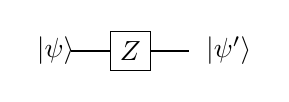
\begin{tikzpicture}
            \draw  (0,0) rectangle (0.5,0.5);
            \node at (0.25,0.25) {$Z$};
            \draw[thick] (-0.5,0.25) -- (0,0.25);
            \draw[thick] (0.5,0.25) -- (1,0.25);
            \node at (-0.7,0.25) {$\ket{\psi}$};
            \node at (1.5,0.25) {$\ket{\psi'}$};
        \end{tikzpicture} 
        & 
        $\begin{bmatrix} 
        1 & 0 \\ 
        0 & -1 
        \end{bmatrix}$ & 
        $\ket{\psi'} = \alpha\ket{0} - \beta\ket{1}$
        \\ \hline

        
    \end{tabular}
    
    \label{tab:quantum_gates}
\end{table*}
\subsection{Quantum Circuit Model}
The key components of a quantum circuit as illustrated in Fig. \ref{fig:QuantumCircuitModel} are:
\begin{enumerate}
    \item \textbf{Classical Resources:} Quantum circuit can be considered to be divided into two parts: Classical part and Quantum part. The true strength of a quantum system is harnessed by leveraging the strengths of both the computation paradigms and integrating both the systems.
    \item \textbf{State Space:} Similar to bits in classical systems, quantum computers work on a number of qubits. The qubits occupy a state space , which is a $2^n$ dimensional Hilbert Space, where n is the number of Qubits.    
    
    A computational basis state $\ket{x}$ corresponds to the binary number $x$ where 
    \begin{center}
    $\ket{x}=\ket{x_1,x_2,...,x_n}$ ,\\  
    $x=x_1 x_2 ..nx_n$ and  \\$x_i=0,1$    
    \end{center}
    \item \textbf{Prepare the state space:} The computational basis states $\ket{x_1,x_2,...,x_n}$ are prepared in atmost $n$ steps.

    \item \textbf{Apply gates and compute:} Once the system is in its initial state, Quantum gates are applides to the required Qubits as per the model/ problem solution and computations are preformed.

    \item \textbf{Measure the results:} After the computations, the results are measured in the computational basis state $\ket{x_i}$. The results are measured classically as $x_i$ corresponding to $\ket{x_i}$
\end{enumerate}
Model is illustrated in Fig.\ref{fig:QuantumCircuitModel} 
\begin{figure*}[tbp]
    \centering
     
    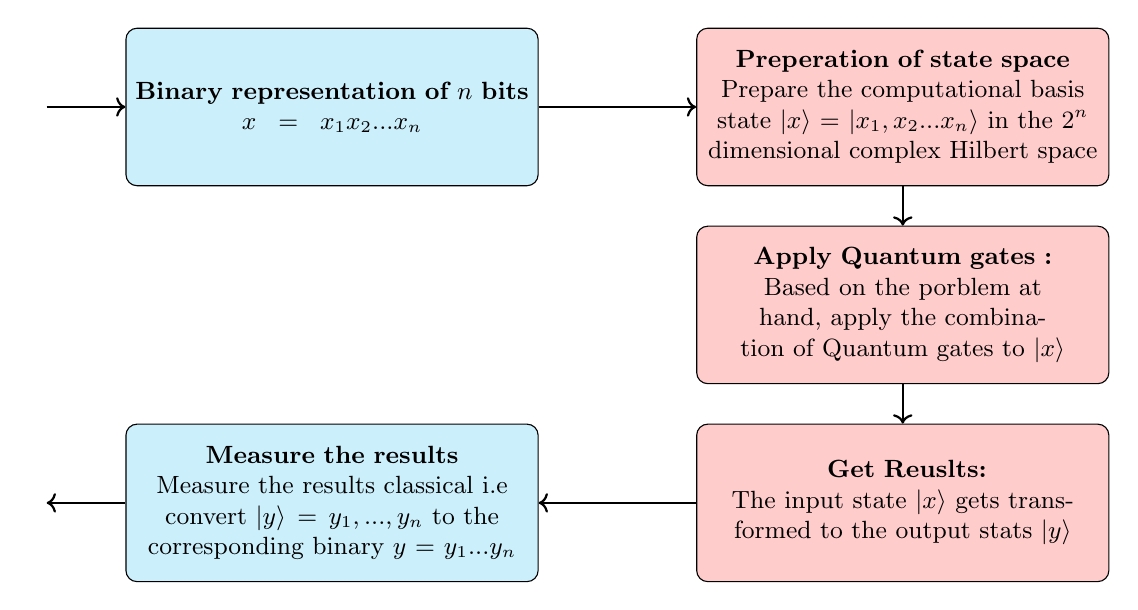
\begin{tikzpicture}[
    box/.style={rectangle, draw, rounded corners, align=center, text width=5cm, minimum height=2cm, font=\small},
    phase/.style={draw, rounded corners, thick, align=center, minimum height=2cm, text width=12cm} ,    
    fillBox/.style={rectangle, fill=red!5, draw, minimum width=5cm, minimum height=2cm, text centered }]
           
        \node[box, draw=black, fill=cyan!20] (QStep1) {\textbf{Binary representation of $n$ bits} \\$x=x_1 x_2 ... x_n$};
        
        \node[box, draw=black, below=0.5cm of QStep1 , fill=red!20 , right=2cm of QStep1] (QStep2) {\textbf{Preperation of state space} Prepare the computational basis state $\ket{x}=\ket{x_1,x_2...x_n}$ in the $2^n$ dimensional complex Hilbert space };
        
        \node[box, draw=black, below=0.5cm of QStep2 , fill=red!20] (QStep3){\textbf{Apply Quantum gates :}\\Based on the porblem at hand, apply the combination of Quantum gates to $\ket{x}$};
        
            
        \node[box, draw=black, below=0.5cm of QStep3 , fill=red!20] (QStep4) {\textbf{
        Get Reuslts:}\\The input state $\ket{x}$ gets transformed to the output stats $\ket{y}$};
        
        \node[box, draw=black,  left =2 cm of QStep4 , fill=cyan!20](QStep5) {\textbf{Measure the results}\\Measure the results classical i.e convert $\ket{y}={y_1, ... ,y_n}$ to the corresponding binary $y=y_1 ... y_n$};               
         
        \draw[->, thick] ( QStep1) -- ( QStep2);
        %\draw[->, thick] (QStep2) -- (QStep1);
        \draw[->, thick] (QStep2) -- (QStep3);
        \draw[->, thick] ( QStep3) -- (QStep4);
        \draw[->, thick] (  QStep4) -- (QStep5);       
       
    \node[left = of QStep1](foo){};
    \node[left = of QStep5](eoo){};
        
        \draw[->, thick] (foo) -- (QStep1) ;
        \draw[->, thick] (QStep5) -- (eoo) ;         
    
    \end{tikzpicture}
   
    
    \caption{ Quantum Circuit Model}
    \label{fig:QuantumCircuitModel}
\end{figure*}

\section{Machine Learning}

Machine learning tries to mimic the human nature of learning from past experiences to react to new stimuli. What this means is, based all the past data collected, a model is developed which then gives a prediction of the outcome. The prediction is probabilistic and rarely 100\% accurate. Machine learning involves seven steps\cite{7} as shown in Fig. \ref{fig:MLSteps} .

\begin{figure*}[t]
    \centering
      
    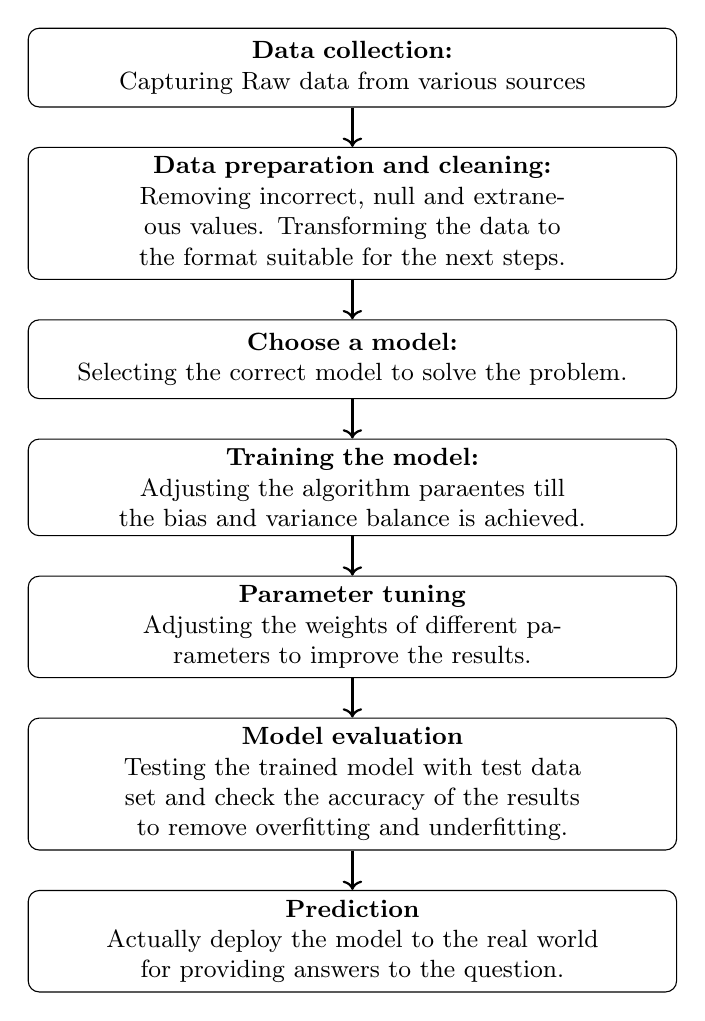
\begin{tikzpicture}[
    box/.style={rectangle, draw, rounded corners, align=center, text width=8cm, minimum height=1cm, font=\small},
    phase/.style={draw, rounded corners, thick, inner sep=0.5cm, minimum height=10cm, minimum width=10cm}]

        % First column
        %\node[phase, label=above:Machine Learning Steps] (Machine Learning Steps) {};
        \node[box, draw=black] (Step1) {\textbf{Data collection:} \\Capturing Raw data from various sources};
        \node[box, draw=black, below=0.5cm of Step1 ] (Step2) {\textbf{Data preparation and cleaning:}\\ Removing incorrect, null and extraneous values. Transforming the data to the format suitable for the next steps.};
        \node[box, draw=black, below=0.5cm of Step2] (Step3){\textbf{Choose a model:}\\Selecting the correct model to solve the problem.} ;
        \node[box, draw=black, below=0.5cm of Step3] (Step4) {\textbf{Training the model:}\\Adjusting the algorithm paraentes till the bias and variance balance is achieved.};
        \node[box, draw=black, below=0.5cm of Step4] (Step5) {\textbf{Parameter tuning}\\Adjusting the weights of different parameters to improve the results.};
        \node[box, draw=black, below=0.5cm of Step5] (Step6) {\textbf{Model evaluation}\\Testing the trained model with test data set and check the accuracy of the results to remove overfitting and underfitting.};
        \node[box, draw=black, below=0.5cm of Step6] (Step7) {\textbf{Prediction}\\Actually deploy the model to the real world for providing answers to the question.};
        \draw[->, thick] (Step1) -- (Step2);
        \draw[->, thick] (Step2) -- (Step3);
        \draw[->, thick] (Step3) -- (Step4);
        \draw[->, thick] (Step4) -- (Step5);
        \draw[->, thick] (Step5) -- (Step6);
        \draw[->, thick] (Step6) -- (Step7);
    
    \end{tikzpicture}
    
    \caption{Machine Learning Steps}
    \label{fig:MLSteps}
\end{figure*}

\section{Quantum Machine Learning(QML)}
\subsection{Introduction to QML}
Machine learning relies heavily on probabilities. This is what makes Quantum systems a good candidate for machine learning application as Quantum Computing also, basically relies on calculating the probability of getting to a particular state.  
Quantum computers due their strength in handling vast quantities of data and parallel processing \cite{7} by Deutch Algorithm, can aid in machine learning tasks. 
The power of Quantum computing can  be leveraged in Machine learning to give 4 combinations of approaches:
The work done in \cite{8} discusses these 4 approaches as shown in Table \ref{tab:QMLApproaches}:

\begin{table*}[p]
    \centering
    \caption{Different approaches to QML}
    \renewcommand{\arraystretch}{3.5} % for row height
    \begin{tabular}{|p{3cm}|p{3cm}|p{4cm}|p{3cm}|}
        \hline
        \textbf{Approach} & \textbf{Concept} & \textbf{Working} & \textbf{Example} \\ \hline
        \multirow{2}{3cm}{Classical-Classical \\ (CC):} & \multirow{2}{3cm}{These are regular algorithms that take inspiration from quantum mechanics.} & \multirow{2}{3.5cm}{They run on normal computers and work with everyday data, but use ideas from quantum computing to improve performance.} & Algorithms designed based on quantum concepts, like optimization techniques that mimic quantum behavior but run on classical systems. \\ \hline
        
        \multirow{2}{3cm}{Classical-Quantum \\ (CQ):} & \multirow{2}{3cm}{Here, quantum computing is used to process traditional (classical) data.} & \multirow{2}{3.5cm}{Quantum algorithms, or adaptations of existing machine learning algorithms, are applied to classical data in a way that aims to outperform regular computer algorithms.} & A quantum version of a neural network that processes data like images or text, hoping to solve problems faster than classical computers. \\ \hline
        
        \multirow{2}{3cm}{Quantum-Classical \\ (QC):} & \multirow{2}{3cm}{Classical machine learning is used to make sense of quantum data.} & \multirow{2}{3.5cm}{Quantum computers generate complex quantum data, and then classical machine learning algorithms are used to analyze this data to extract useful information.} & Using traditional machine learning techniques to predict the behavior of quantum systems based on quantum data. \\ \hline
        \multirow{2}{3cm}{Quantum-Quantum \\ (QQ):} & \multirow{2}{3cm}{Both the algorithms and the data are purely quantum.} & \multirow{2}{3.5cm}{Quantum algorithms work directly with quantum data to find patterns or insights, making full use of quantum states.} & A quantum algorithm designed to learn from quantum states for tasks like optimizing quantum systems or recognizing quantum patterns. \\ \hline
    \end{tabular}    
    \label{tab:QMLApproaches}
\end{table*}

The choice of using the classical approach or quantum  approach requires some analysis. As mentioned before, quantum computing algorithms give a clear advantage over classical systems for algorithms with very high sample complexity\cite{bib37} . Quantum approaches due to their probabilistic nature sometimes are more robust to noise than classical algorithms. \cite{cross2015quantum,bshouty1995learning}. Some metrics used in quantum - classical model selection  are computational complexity, sample complexity, robustness to noise, circuit depth (number of layers),accuracy and optimum bias variance tradeoff.\cite{hastie2009high}.

The most common approach for implementing QML is the the CQ setting. The two ways to implement QML is the CQ setting are\cite{bib37} :
\begin{itemize}
    \item The translational approach: Some parts of the classical algorithms are translated i.e. run using Quantum approaches. The choice of using classical or quantum approach is which approach will give better performance (accuracy or speed wise).
    \item  The exploratory approach: The algorithms are run entirely on quantum systems and may not have any quantum counterpart.
\end{itemize}

\subsection{Quantum Data Encoding}\label{QuantumDataEncoding}
 The work done in \cite{Rath2024},\cite{10201947} discuss the quantum data encoding methods used to prepare the data to be input to a machine learning algorithm.
 The three approaches discussed are:
 \subsubsection{Basis Encoding}
 In this method the qubits are directly mapped to the bit values i.e. bit 0 and  1 will be represented as $\ket{0}$ and  $\ket{1}$ respectively.  A classical number 110 can be represented as the quantum state $\ket{110}$:

\begin{equation}
\ket{110} = \alpha \ket{1} \otimes \beta \ket{1} \otimes \gamma \ket{0},
\end{equation}

where $\alpha$, $\beta$, and $\gamma$ are the information stored in the form of probability amplitudes for each qubit state. 

 \subsubsection{Superposition encoding}
As the name suggests, in this encoding scheme, the qubit state is encoded as a superposition of the basis states.

\begin{equation}
\ket{110} = \sqrt{\frac{1}{3}} \ket{100} + \sqrt{\frac{1}{3}} \ket{010} + \sqrt{\frac{1}{3}} \ket{001},
\end{equation}

\begin{equation}
\ket{78} = \sqrt{\frac{1}{2}} \ket{1001110} + \sqrt{\frac{1}{2}} \ket{0100111},
\end{equation}

\subsubsection{Angle encoding}
When the Qubits are represented on the bloch sphere, the probabilities of basis states are the phase shift from the X,Y and Z axes. Thus in angle encoding, the classical data is represented as a phase shift. Quantum gates use rotation operations around different axes (X, Y, or Z) for changing the quantum state.

The rotation around the X, Y and Z axis   denoted as $R_x(\theta)$,$R_y(\theta)$ and $R_y(\theta)$ respectively and is  shown in Equations \ref{eq:Rx},\ref{eq:Ry} and \ref{eq:Rz}. 

\begin{equation}
R_x(\theta) = e^{-i \theta X / 2} = 
\begin{bmatrix}
\cos(\theta / 2) & -i \sin(\theta / 2) \\
-i \sin(\theta / 2) & \cos(\theta / 2)
\end{bmatrix}
\label{eq:Rx}
\end{equation}


\begin{equation}
R_y(\theta) = e^{-i \theta Y / 2} = 
\begin{bmatrix}
\cos(\theta / 2) & -\sin(\theta / 2) \\
\sin(\theta / 2) & \cos(\theta / 2)
\end{bmatrix}
\label{eq:Ry}
\end{equation}

\begin{equation}
R_z(\theta) = e^{-i \theta Z / 2} = 
\begin{bmatrix}
e^{-i \theta / 2} & 0 \\
0 & e^{i \theta / 2}
\end{bmatrix}
\label{eq:Rz}
\end{equation}

\subsubsection{Amplitude encoding}
In this scheme, classical information is encoded in the probability amplitudes of quantum state. If the number of  values to be represented is n, then the number of qubits required are  $ log_2(n)$ . The values of probabilities of each qubit state is the square root of the data value divided by the square root of the sum of squares of all the n data values. The quantum state can be represented as:
\begin{equation}
\ket{\psi(X)} = \sum_{i=1}^n x_i |i\rangle
\end{equation}

where \( x_i \) is the \(i\)-th element of the vector \( X \), and \( |i\rangle \) denotes the computational basis states of the qubits. For this example, \( n = 4 \), and the coefficients \( x_i \) correspond to the values \( [1.2, 2.7, 1.1, 0.5] \).

Each term is square-normalized by dividing it by the square root of the sum of squares of all elements. For the vector \( X = [1.2, 2.7, 1.1, 0.5] \), the normalization factor is:
\begin{equation}
    \sqrt{\sum_{i=1}^n x_i^2} = \sqrt{1.2^2 + 2.7^2 + 1.1^2 + 0.5^2} = \sqrt{10.19}
\end{equation}



The normalized quantum state is:
\begin{align}
|\psi\rangle &= \frac{\sqrt{1.2}}{\sqrt{10.19}} |00\rangle 
+ \frac{\sqrt{2.7}}{\sqrt{10.19}} |01\rangle \nonumber \\
&\quad + \frac{\sqrt{1.1}}{\sqrt{10.19}} |10\rangle 
+ \frac{\sqrt{0.5}}{\sqrt{10.19}} |11\rangle.
\end{align}

\section{Implementation of QML Algorithms}
In their work \cite{rath2023quantum},the authors have suggested the framework to implement Hybrid Quantum Classical algorithms. As discussed previously, Quantum computing can work in tandem with classical system in 4 ways i.e. CC,QC,CQ and QQ.  Normally, a hybrid quantum algorithm contains 3 parts: the classical part,quantum part and the interface between the classical and quantum systems as shown in Fig.\ref{fig:QuantumPartSteps} The data encoding, application of Oracle, amplitude adjustment and Optimization steps are repeated multiple times in the range of thousands of iterations to give reliable results. 


\begin{figure*}[p]
    \centering
    \begin{adjustbox}{width=\textwidth, height=0.9\textheight, keepaspectratio}
         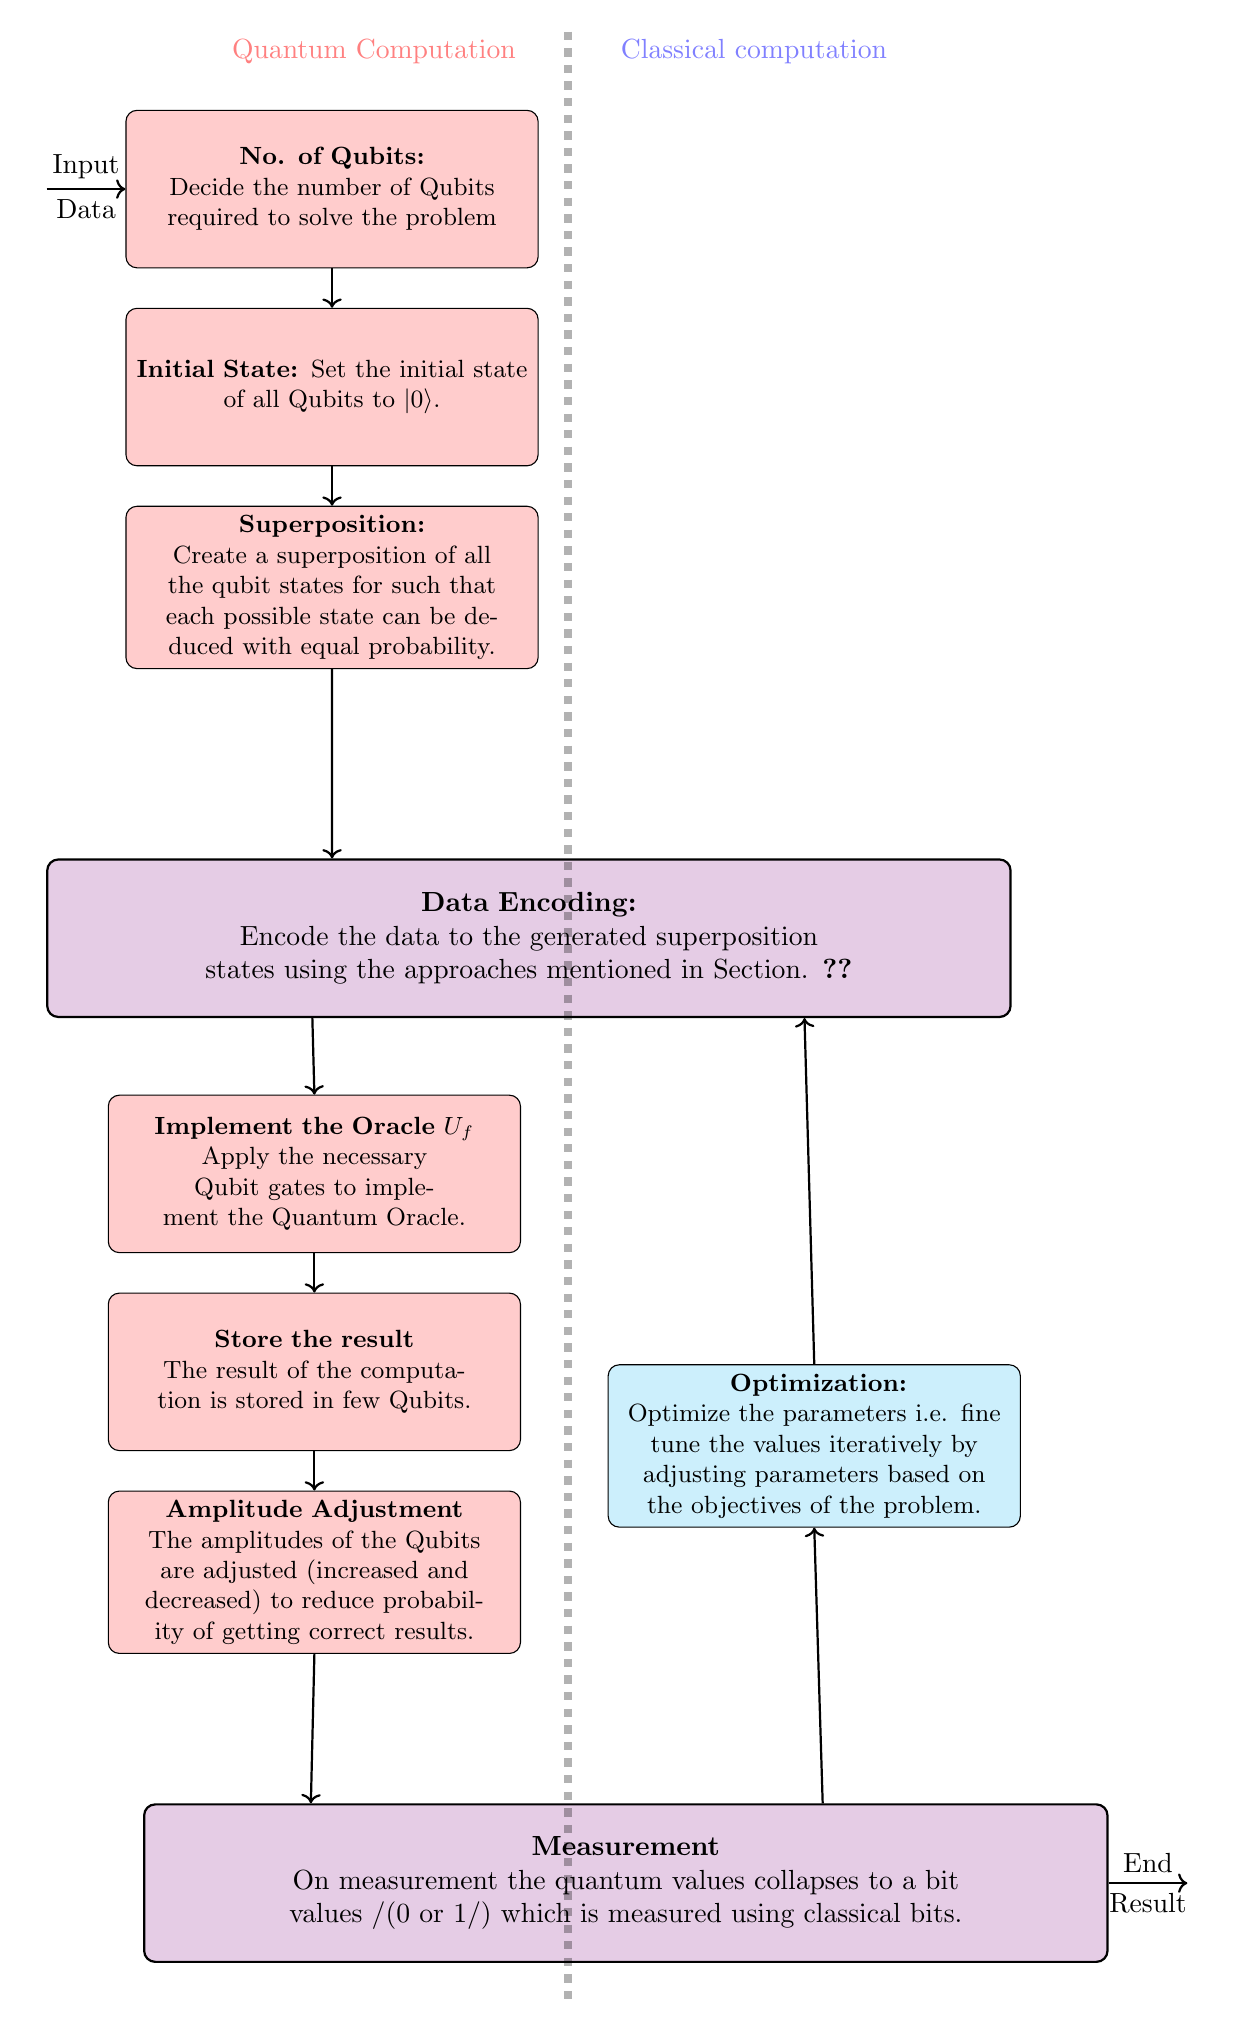
\begin{tikzpicture}[
    box/.style={rectangle, draw, rounded corners, align=center, text width=5cm, minimum height=2cm, font=\small},
    phase/.style={draw, rounded corners, thick, align=center, minimum height=2cm, text width=12cm} ,    
    fillBox/.style={rectangle, fill=red!5, draw, minimum width=5cm, minimum height=2cm, text centered }]
    %\node[fillBox, minimum width=3cm, minimum height=1.5cm] (box1) at (0, 0) {This box is customized};
            % First column
       
        \node[box, draw=black, fill=red!20] (QStep1) {\textbf{No. of Qubits:} \\Decide the number of Qubits required to solve the problem};
        
        \node[box, draw=black, below=0.5cm of QStep1 , fill=red!20] (QStep2) {\textbf{Initial State:} Set the initial state\\ of all Qubits to $\ket{0}$.};
        
        \node[box, draw=black, below=0.5cm of QStep2 , fill=red!20] (QStep3){\textbf{Superposition:}\\Create a superposition of all the qubit states for such that each possible state can be deduced with equal probability.};
        
        %\node[box, draw=black, below=0.5cm of QStep3] (QStep4) {\textbf{Data Encoding:}\\Encode the data to the generated superposition states using the approaches mentioned in Section. \ref{QuantumDataEncoding}};
        
        \node[phase,draw=black, below=0.5cm of QStep3 , fill=violet!20] (QStep4) at (2.5,-8){\textbf{Data Encoding:}\\Encode the data to the generated superposition states using the approaches mentioned in Section. \ref{QuantumDataEncoding}};
        
        \node[box, draw=black, below left =1.5cm and 0.1cm of QStep4 , fill=red!20] at(2.5,-10)(QStep5) {\textbf{Implement the Oracle $U_f$}\\Apply the necessary Qubit gates to implement the Quantum Oracle.};
        
        \node[box, draw=black, below=0.5cm of QStep5 , fill=red!20] (QStep6) {\textbf{Store the result}\\The result of the computation is stored in few Qubits.};
        
        \node[box, draw=black, below =0.5cm  of QStep6 , fill=red!20] (QStep7) {\textbf{Amplitude Adjustment}\\The amplitudes of the Qubits are adjusted (increased and decreased) to reduce probability of getting correct results.};
        
        \node[phase, draw=black, below right=0.5cm and 0.1cm of QStep7 , fill=violet!20] (QStep8) at (-2.5,-20){\textbf{Measurement}\\On measurement the quantum values collapses to a bit values /(0 or 1/) which is measured using classical bits.};
         
        \draw[->, thick] ( QStep1) -- ( QStep2);
        %\draw[->, thick] (QStep2) -- (QStep1);
        \draw[->, thick] (QStep2) -- (QStep3);
        \draw[->, thick] ( QStep3.south) -- ([xshift=-2.5cm]QStep4.north);
        \draw[->, thick] ( [xshift=-2.75cm] QStep4.south) -- (QStep5.north);
        \draw[->, thick] (QStep5) -- (QStep6);
        \draw[->, thick] (QStep6) -- (QStep7);
        \draw[->, thick] (QStep7.south) -- ([xshift=-4cm] QStep8.north);


       % \node[box, draw=black, right=0.5cm of QStep8] (CStep1) {\textbf{Measurement:} \\On measurement the quantum values collapse to a bit values /(0 or 1/) which is measured and stored as classical bits in binary registers.};
        \node[box, draw=black,above right=2cm and 0cm of QStep8 , fill=cyan!20] (CStep2) at (3.5,-19){\textbf{
Optimization:}\\ Optimize the parameters i.e. fine tune  the values iteratively by adjusting parameters based on the objectives of the problem.};

  %  \node[box, draw=black, above=0.5cm of CStep2] (CStep3){\textbf{Quantum Encoding:}\\Encode the bits back to Quantum bits.} ;


    \node[left = of QStep1](foo){};
    \node[right = of QStep8](eoo){};

        \draw[->, thick] ([xshift=2.5cm]QStep8.north) -- (CStep2.south);
      %   \draw[->, thick] (CStep1) -- (CStep2);
        \draw[->, thick] (CStep2.north) -- ([xshift=3.5cm]QStep4.south);

       % \draw[->, thick] (CStep3) -- (QStep4);

        \draw[->, thick] (foo) -- node[above] {Input} node[below]{Data}(QStep1);
        \draw[->, thick] (QStep8) --node[above] {End}node[below]{ Result} (eoo);     



    \draw[dashed, opacity=0.3,line width=1mm] 
        (3,2) 
        -- 
        node[pos=0.01, left, xshift=-5mm, text=red!50, opacity=1] {Quantum Computation} 
        node[pos=0.01, right, xshift=5mm, text = blue!50, opacity=1] {Classical computation} 
        (3,-23);    
    \end{tikzpicture}     
     \end{adjustbox}
    \caption{ Framework to implement the Quantum Machine learning.}
    \label{fig:QuantumPartSteps}
\end{figure*}



\subsection{Quantum Computation}
The quantum part comprises of mapping the algorithm to an actual circuit with quantum gates.
The steps involved in this process, shown on the left side of Fig. \ref{fig:QuantumPartSteps} in red, are:

\begin{enumerate}
    \item Decide the number of qubits required and set them to the basis state of $\ket{0}$.
    \item Apply the Hadamard Gate to create a uniform superposition of all possible states of the qubits.
    \item Encode the the resultant states using any of the encoding techniques mentioned in \ref{QuantumDataEncoding}.
    \item Apply quantum gates to implement the Quantum Oracle function ($U_f$ ) on the encoded qubits. 
    \item The result after applying the Oracle function is stored in all or few of the Qubits.
    \item The amplitudes of the undesired states are  reduced to increase the probability of the getting the desired result.
    
    \item The final values are measured. As discussed earlier, on measurement, the state of a Qubits collapses to classical bit value. The binary value will depend on the probability of each state.
    
\end{enumerate}
\subsection{Classical Computation}
In the classical component, classical values obtained are optimised using classical techniques.
The steps involved, shown on the right hand side of Fig. \ref{fig:QuantumPartSteps} in cyan, are:
\begin{enumerate}
    \item The final qubit values are measured classically.The binary value obtained on measurement will depend on the quantum probability of each state.
    \item In this step, the values are iteratively modified based on the problem statement and expected results. This is done to increase the probability of correct results. Error correction and mitigation strategies are applied for better results.
   
\end{enumerate}

\subsection{Interface between Quantum and Classical systems}
This phase is shown in Fig. \ref{fig:QuantumPartSteps} in the violet boxes.
\begin{enumerate}
    \item Data Encoding: The binary bits are encoded using any one of the encoding techniques discussed in Section \ref{QuantumDataEncoding}.
    \item Measurement: The Qubits are measured where they take a binary value of 0 or 1. 
\end{enumerate}


\section{Tools available for Quantum Computing}
Quantum computing has opened doors to solving the problems earlier considered unsolvable. This also poses a threat to our existing system security. All this has sparked a keen interest in Quantum research. A number of tools are  available to develop and run quantum algorithms. Some of the tools are tabulated in Table \ref{tab:QuantumDevelopmentToolKits}.

\begin{table}
    \centering
    \caption{Quantum Development Toolkits}
    \begin{tabular}{|p{1.5cm}|p{2cm}|p{2cm}|p{2cm}|}
    \hline
    \textbf{SDK / Library} & \textbf{Language} & \textbf{Hardware} & \textbf{Platform / Cloud Service} \\ \hline

    \textbf{IBM Qiskit} \cite{aleksandrowicz2019qiskit} 
    & Python 
    & IBM Quantum hardware 
    & IBM Quantum Experience \\ \hline

    \textbf{Google Cirq} \cite{quantumaiCirqGoogle}
    & Python 
    & Google’s quantum hardware 
    & Google Quantum AI \\ \hline

    \textbf{Ms QDK} \cite{svore2018q}
    & Q$\#$ 
    & Supports multiple hardware providers through Azure 
    & Azure Quantum \\ \hline

    \textbf{Rigetti Forest} \cite{smith2016practical} 
    & PyQuil 
    & Rigetti’s superconducting quantum processors 
    & Rigetti Quantum Cloud \\ \hline

    \textbf{Tensor Flow Quantum} \cite{broughton2020tensorflow} 
    & Python 
    & Works on quantum hardware using the Cirq library 
    & TensorFlow ecosystem \\ \hline

    \textbf{Xanadu PennyLane} \cite{bergholm2018pennylane} 
    & Python 
    & Xanadu’s photonic processors 
    & Xanadu Cloud \\ \hline

    \textbf{D-Wave Ocean SDK} \cite{dwavesysDWaveOcean}
    & Python 
    & D-Wave quantum computers 
    & Leap Quantum Cloud \\ \hline

    \textbf{Open Fermion} \cite{quantumaiOpenFermionGoogle}
    & Python 
    & Compatible with Cirq, Qiskit, and other frameworks 
    & Not platform-specific \\ \hline

    \textbf{Amazon Braket} \cite{amazonBraket} 
    & Python 
    & Multiple QPUs and simulators 
    & Amazon Web Services \\ \hline
    \end{tabular}
    
    \label{tab:QuantumDevelopmentToolKits}
\end{table}

\section{Conclusion}
Quantum computing is more than just a breakthrough in technology—it’s a whole new way of thinking about how we solve problems. By harnessing the strange yet powerful properties of quantum mechanics, quantum computers can tackle challenges that classical systems simply can’t handle. From optimizing complex systems to analyzing massive datasets, the potential impact on industries like healthcare, finance, and artificial intelligence is staggering. But this isn’t a technology we’ll see in full force tomorrow. Building practical quantum computers is hard. Qubits, the building blocks of quantum systems, are delicate and prone to errors. Scaling up to larger, more reliable systems will take time and innovation. Even so, companies like IBM and Google have already made impressive strides with powerful quantum processors. Meanwhile, cloud platforms like Amazon Braket and Microsoft Azure Quantum are making quantum computing tools accessible to more people, speeding up the pace of discovery and development.

In machine learning, quantum computing offers unique ways to improve existing algorithms and solve new types of problems. Hybrid systems—where quantum and classical computers work together—are showing how these two worlds can complement each other. Libraries and frameworks, like Qiskit and TensorFlow Quantum, are making it easier for developers and researchers to experiment with quantum ideas in practical ways.

The potential of quantum computing is undeniable despite the numerous challenges. The future of quantum computing will depend not only on solving technical problems but also on collaborations across science, industry, and policymaking. It’s a journey, but one filled with incredible promise. If progress continues at its current pace, quantum computing could soon transform the way we live, work, and think about technology.

%\bibliographystyle{quantum}
\bibliographystyle{plainnat}
\bibliography{bibliography}
%\printbibliography
\end{document}